
%% bare_adv.tex
%% V1.4
%% 2012/12/27
%% by Michael Shell
%% See: 
%% http://www.michaelshell.org/
%% for current contact information.
%%
%% This is a skeleton file demonstrating the advanced use of IEEEtran.cls
%% (requires IEEEtran.cls version 1.8 or later) with an IEEE Computer
%% Society journal paper.
%%
%% Support sites:
%% http://www.michaelshell.org/tex/ieeetran/
%% http://www.ctan.org/tex-archive/macros/latex/contrib/IEEEtran/
%% and
%% http://www.ieee.org/

%%*************************************************************************
%% Legal Notice:
%% This code is offered as-is without any warranty either expressed or
%% implied; without even the implied warranty of MERCHANTABILITY or
%% FITNESS FOR A PARTICULAR PURPOSE! 
%% User assumes all risk.
%% In no event shall IEEE or any contributor to this code be liable for
%% any damages or losses, including, but not limited to, incidental,
%% consequential, or any other damages, resulting from the use or misuse
%% of any information contained here.
%%
%% All comments are the opinions of their respective authors and are not
%% necessarily endorsed by the IEEE.
%%
%% This work is distributed under the LaTeX Project Public License (LPPL)
%% ( http://www.latex-project.org/ ) version 1.3, and may be freely used,
%% distributed and modified. A copy of the LPPL, version 1.3, is included
%% in the base LaTeX documentation of all distributions of LaTeX released
%% 2003/12/01 or later.
%% Retain all contribution notices and credits.
%% ** Modified files should be clearly indicated as such, including  **
%% ** renaming them and changing author support contact information. **
%%
%% File list of work: IEEEtran.cls, IEEEtran_HOWTO.pdf, bare_adv.tex,
%%                    bare_conf.tex, bare_jrnl.tex, bare_jrnl_compsoc.tex,
%%                    bare_jrnl_transmag.tex
%%*************************************************************************

% *** Authors should verify (and, if needed, correct) their LaTeX system  ***
% *** with the testflow diagnostic prior to trusting their LaTeX platform ***
% *** with production work. IEEE's font choices can trigger bugs that do  ***
% *** not appear when using other class files.                            ***
% The testflow support page is at:
% http://www.michaelshell.org/tex/testflow/



% IEEEtran V1.7 and later provides for these CLASSINPUT macros to allow the
% user to reprogram some IEEEtran.cls defaults if needed. These settings
% override the internal defaults of IEEEtran.cls regardless of which class
% options are used. Do not use these unless you have good reason to do so as
% they can result in nonIEEE compliant documents. User beware. ;)
%
%\newcommand{\CLASSINPUTbaselinestretch}{1.0} % baselinestretch
%\newcommand{\CLASSINPUTinnersidemargin}{1in} % inner side margin
%\newcommand{\CLASSINPUToutersidemargin}{1in} % outer side margin
%\newcommand{\CLASSINPUTtoptextmargin}{1in}   % top text margin
%\newcommand{\CLASSINPUTbottomtextmargin}{1in}% bottom text margin



% Note that the a4paper option is mainly intended so that authors in
% countries using A4 can easily print to A4 and see how their papers will
% look in print - the typesetting of the document will not typically be
% affected with changes in paper size (but the bottom and side margins will).
% Use the testflow package mentioned above to verify correct handling of
% both paper sizes by the user's LaTeX system.
%
% Also note that the "draftcls" or "draftclsnofoot", not "draft", option
% should be used if it is desired that the figures are to be displayed in
% draft mode.
%
\documentclass[12pt,journal,compsoc]{IEEEtran}
% The Computer Society requires 12pt.
% If IEEEtran.cls has not been installed into the LaTeX system files,
% manually specify the path to it like:
% \documentclass[10pt,journal,compsoc]{../sty/IEEEtran}


% For Computer Society journals, IEEEtran defaults to the use of 
% Palatino/Palladio as is done in IEEE Computer Society journals.
% To go back to Times Roman, you can use this code:
%\renewcommand{\rmdefault}{ptm}\selectfont





% Some very useful LaTeX packages include:
% (uncomment the ones you want to load)



% *** MISC UTILITY PACKAGES ***
%
%\usepackage{ifpdf}
% Heiko Oberdiek's ifpdf.sty is very useful if you need conditional
% compilation based on whether the output is pdf or dvi.
% usage:
% \ifpdf
%   % pdf code
% \else
%   % dvi code
% \fi
% The latest version of ifpdf.sty can be obtained from:
% http://www.ctan.org/tex-archive/macros/latex/contrib/oberdiek/
% Also, note that IEEEtran.cls V1.7 and later provides a builtin
% \ifCLASSINFOpdf conditional that works the same way.
% When switching from latex to pdflatex and vice-versa, the compiler may
% have to be run twice to clear warning/error messages.






% *** CITATION PACKAGES ***
%
\ifCLASSOPTIONcompsoc
  % IEEE Computer Society needs nocompress option
  % requires cite.sty v4.0 or later (November 2003)
  % \usepackage[nocompress]{cite}
\else
  % normal IEEE
  % \usepackage{cite}
\fi
% cite.sty was written by Donald Arseneau
% V1.6 and later of IEEEtran pre-defines the format of the cite.sty package
% \cite{} output to follow that of IEEE. Loading the cite package will
% result in citation numbers being automatically sorted and properly
% "compressed/ranged". e.g., [1], [9], [2], [7], [5], [6] without using
% cite.sty will become [1], [2], [5]--[7], [9] using cite.sty. cite.sty's
% \cite will automatically add leading space, if needed. Use cite.sty's
% noadjust option (cite.sty V3.8 and later) if you want to turn this off
% such as if a citation ever needs to be enclosed in parenthesis.
% cite.sty is already installed on most LaTeX systems. Be sure and use
% version 4.0 (2003-05-27) and later if using hyperref.sty. cite.sty does
% not currently provide for hyperlinked citations.
% The latest version can be obtained at:
% http://www.ctan.org/tex-archive/macros/latex/contrib/cite/
% The documentation is contained in the cite.sty file itself.
%
% Note that some packages require special options to format as the Computer
% Society requires. In particular, Computer Society  papers do not use
% compressed citation ranges as is done in typical IEEE papers
% (e.g., [1]-[4]). Instead, they list every citation separately in order
% (e.g., [1], [2], [3], [4]). To get the latter we need to load the cite
% package with the nocompress option which is supported by cite.sty v4.0
% and later.
%
% Note also the use of a CLASSOPTION conditional provided by 
% IEEEtran.cls V1.7 and later.





% *** GRAPHICS RELATED PACKAGES ***
%
\ifCLASSINFOpdf
  \usepackage[pdftex]{graphicx}
  % declare the path(s) where your graphic files are
  \graphicspath{{/home/saf537/Documents/CUSP/Capstone/Bus-Capstone/plots}}
  % and their extensions so you won't have to specify these with
  % every instance of \includegraphics
  \DeclareGraphicsExtensions{.pdf,.jpeg,.png}
\else
  % or other class option (dvipsone, dvipdf, if not using dvips). graphicx
  % will default to the driver specified in the system graphics.cfg if no
  % driver is specified.
  \usepackage[dvips]{graphicx}
  % declare the path(s) where your graphic files are
  \graphicspath{{/home/saf537/Documents/CUSP/Capstone/Bus-Capstone/plots}}
  % and their extensions so you won't have to specify these with
  % every instance of \includegraphics
  % \DeclareGraphicsExtensions{.eps}
\fi
% graphicx was written by David Carlisle and Sebastian Rahtz. It is
% required if you want graphics, photos, etc. graphicx.sty is already
% installed on most LaTeX systems. The latest version and documentation
% can be obtained at: 
% http://www.ctan.org/tex-archive/macros/latex/required/graphics/
% Another good source of documentation is "Using Imported Graphics in
% LaTeX2e" by Keith Reckdahl which can be found at:
% http://www.ctan.org/tex-archive/info/epslatex/
%
% latex, and pdflatex in dvi mode, support graphics in encapsulated
% postscript (.eps) format. pdflatex in pdf mode supports graphics
% in .pdf, .jpeg, .png and .mps (metapost) formats. Users should ensure
% that all non-photo figures use a vector format (.eps, .pdf, .mps) and
% not a bitmapped formats (.jpeg, .png). IEEE frowns on bitmapped formats
% which can result in "jaggedy"/blurry rendering of lines and letters as
% well as large increases in file sizes.
%
% You can find documentation about the pdfTeX application at:
% http://www.tug.org/applications/pdftex





% *** MATH PACKAGES ***
%
%\usepackage[cmex10]{amsmath}
% A popular package from the American Mathematical Society that provides
% many useful and powerful commands for dealing with mathematics. If using
% it, be sure to load this package with the cmex10 option to ensure that
% only type 1 fonts will utilized at all point sizes. Without this option,
% it is possible that some math symbols, particularly those within
% footnotes, will be rendered in bitmap form which will result in a
% document that can not be IEEE Xplore compliant!
%
% Also, note that the amsmath package sets \interdisplaylinepenalty to 10000
% thus preventing page breaks from occurring within multiline equations. Use:
%\interdisplaylinepenalty=2500
% after loading amsmath to restore such page breaks as IEEEtran.cls normally
% does. amsmath.sty is already installed on most LaTeX systems. The latest
% version and documentation can be obtained at:
% http://www.ctan.org/tex-archive/macros/latex/required/amslatex/math/





% *** SPECIALIZED LIST PACKAGES ***
%\usepackage{acronym}
% acronym.sty was written by Tobias Oetiker. This package provides tools for
% managing documents with large numbers of acronyms. (You don't *have* to
% use this package - unless you have a lot of acronyms, you may feel that
% such package management of them is bit of an overkill.)
% Do note that the acronym environment (which lists acronyms) will have a
% problem when used under IEEEtran.cls because acronym.sty relies on the
% description list environment - which IEEEtran.cls has customized for
% producing IEEE style lists. A workaround is to declared the longest
% label width via the IEEEtran.cls \IEEEiedlistdecl global control:
%
% \renewcommand{\IEEEiedlistdecl}{\IEEEsetlabelwidth{SONET}}
% \begin{acronym}
%
% \end{acronym}
% \renewcommand{\IEEEiedlistdecl}{\relax}% remember to reset \IEEEiedlistdecl
%
% instead of using the acronym environment's optional argument.
% The latest version and documentation can be obtained at:
% http://www.ctan.org/tex-archive/macros/latex/contrib/acronym/


%\usepackage{algorithmic}
% algorithmic.sty was written by Peter Williams and Rogerio Brito.
% This package provides an algorithmic environment fo describing algorithms.
% You can use the algorithmic environment in-text or within a figure
% environment to provide for a floating algorithm. Do NOT use the algorithm
% floating environment provided by algorithm.sty (by the same authors) or
% algorithm2e.sty (by Christophe Fiorio) as IEEE does not use dedicated
% algorithm float types and packages that provide these will not provide
% correct IEEE style captions. The latest version and documentation of
% algorithmic.sty can be obtained at:
% http://www.ctan.org/tex-archive/macros/latex/contrib/algorithms/
% There is also a support site at:
% http://algorithms.berlios.de/index.html
% Also of interest may be the (relatively newer and more customizable)
% algorithmicx.sty package by Szasz Janos:
% http://www.ctan.org/tex-archive/macros/latex/contrib/algorithmicx/




% *** ALIGNMENT PACKAGES ***
%
%\usepackage{array}
% Frank Mittelbach's and David Carlisle's array.sty patches and improves
% the standard LaTeX2e array and tabular environments to provide better
% appearance and additional user controls. As the default LaTeX2e table
% generation code is lacking to the point of almost being broken with
% respect to the quality of the end results, all users are strongly
% advised to use an enhanced (at the very least that provided by array.sty)
% set of table tools. array.sty is already installed on most systems. The
% latest version and documentation can be obtained at:
% http://www.ctan.org/tex-archive/macros/latex/required/tools/


%\usepackage{mdwmath}
%\usepackage{mdwtab}
% Also highly recommended is Mark Wooding's extremely powerful MDW tools,
% especially mdwmath.sty and mdwtab.sty which are used to format equations
% and tables, respectively. The MDWtools set is already installed on most
% LaTeX systems. The lastest version and documentation is available at:
% http://www.ctan.org/tex-archive/macros/latex/contrib/mdwtools/


% IEEEtran contains the IEEEeqnarray family of commands that can be used to
% generate multiline equations as well as matrices, tables, etc., of high
% quality.


%\usepackage{eqparbox}
% Also of notable interest is Scott Pakin's eqparbox package for creating
% (automatically sized) equal width boxes - aka "natural width parboxes".
% Available at:
% http://www.ctan.org/tex-archive/macros/latex/contrib/eqparbox/




% *** SUBFIGURE PACKAGES ***
%\ifCLASSOPTIONcompsoc
%  \usepackage[caption=false,font=normalsize,labelfont=sf,textfont=sf]{subfig}
%\else
%  \usepackage[caption=false,font=footnotesize]{subfig}
%\fi
% subfig.sty, written by Steven Douglas Cochran, is the modern replacement
% for subfigure.sty, the latter of which is no longer maintained and is
% incompatible with some LaTeX packages including fixltx2e. However,
% subfig.sty requires and automatically loads Axel Sommerfeldt's caption.sty
% which will override IEEEtran.cls' handling of captions and this will result
% in non-IEEE style figure/table captions. To prevent this problem, be sure
% and invoke subfig.sty's "caption=false" package option (available since
% subfig.sty version 1.3, 2005/06/28) as this is will preserve IEEEtran.cls
% handling of captions.
% Note that the Computer Society format requires a larger sans serif font
% than the serif footnote size font used in traditional IEEE formatting
% and thus the need to invoke different subfig.sty package options depending
% on whether compsoc mode has been enabled.
%
% The latest version and documentation of subfig.sty can be obtained at:
% http://www.ctan.org/tex-archive/macros/latex/contrib/subfig/




% *** FLOAT PACKAGES ***
%
%\usepackage{fixltx2e}
% fixltx2e, the successor to the earlier fix2col.sty, was written by
% Frank Mittelbach and David Carlisle. This package corrects a few problems
% in the LaTeX2e kernel, the most notable of which is that in current
% LaTeX2e releases, the ordering of single and double column floats is not
% guaranteed to be preserved. Thus, an unpatched LaTeX2e can allow a
% single column figure to be placed prior to an earlier double column
% figure. The latest version and documentation can be found at:
% http://www.ctan.org/tex-archive/macros/latex/base/


%\usepackage{stfloats}
% stfloats.sty was written by Sigitas Tolusis. This package gives LaTeX2e
% the ability to do double column floats at the bottom of the page as well
% as the top. (e.g., "\begin{figure*}[!b]" is not normally possible in
% LaTeX2e). It also provides a command:
%\fnbelowfloat
% to enable the placement of footnotes below bottom floats (the standard
% LaTeX2e kernel puts them above bottom floats). This is an invasive package
% which rewrites many portions of the LaTeX2e float routines. It may not work
% with other packages that modify the LaTeX2e float routines. The latest
% version and documentation can be obtained at:
% http://www.ctan.org/tex-archive/macros/latex/contrib/sttools/
% Do not use the stfloats baselinefloat ability as IEEE does not allow
% \baselineskip to stretch. Authors submitting work to the IEEE should note
% that IEEE rarely uses double column equations and that authors should try
% to avoid such use. Do not be tempted to use the cuted.sty or midfloat.sty
% packages (also by Sigitas Tolusis) as IEEE does not format its papers in
% such ways.
% Do not attempt to use stfloats with fixltx2e as they are incompatible.
% Instead, use Morten Hogholm'a dblfloatfix which combines the features
% of both fixltx2e and stfloats:
%
% \usepackage{dblfloatfix}
% The latest version can be found at:
% http://www.ctan.org/tex-archive/macros/latex/contrib/dblfloatfix/


%\ifCLASSOPTIONcaptionsoff
%  \usepackage[nomarkers]{endfloat}
% \let\MYoriglatexcaption\caption
% \renewcommand{\caption}[2][\relax]{\MYoriglatexcaption[#2]{#2}}
%\fi
% endfloat.sty was written by James Darrell McCauley, Jeff Goldberg and 
% Axel Sommerfeldt. This package may be useful when used in conjunction with 
% IEEEtran.cls'  captionsoff option. Some IEEE journals/societies require that
% submissions have lists of figures/tables at the end of the paper and that
% figures/tables without any captions are placed on a page by themselves at
% the end of the document. If needed, the draftcls IEEEtran class option or
% \CLASSINPUTbaselinestretch interface can be used to increase the line
% spacing as well. Be sure and use the nomarkers option of endfloat to
% prevent endfloat from "marking" where the figures would have been placed
% in the text. The two hack lines of code above are a slight modification of
% that suggested by in the endfloat docs (section 8.4.1) to ensure that
% the full captions always appear in the list of figures/tables - even if
% the user used the short optional argument of \caption[]{}.
% IEEE papers do not typically make use of \caption[]'s optional argument,
% so this should not be an issue. A similar trick can be used to disable
% captions of packages such as subfig.sty that lack options to turn off
% the subcaptions:
% For subfig.sty:
% \let\MYorigsubfloat\subfloat
% \renewcommand{\subfloat}[2][\relax]{\MYorigsubfloat[]{#2}}
% However, the above trick will not work if both optional arguments of
% the \subfloat command are used. Furthermore, there needs to be a
% description of each subfigure *somewhere* and endfloat does not add
% subfigure captions to its list of figures. Thus, the best approach is to
% avoid the use of subfigure captions (many IEEE journals avoid them anyway)
% and instead reference/explain all the subfigures within the main caption.
% The latest version of endfloat.sty and its documentation can obtained at:
% http://www.ctan.org/tex-archive/macros/latex/contrib/endfloat/
%
% The IEEEtran \ifCLASSOPTIONcaptionsoff conditional can also be used
% later in the document, say, to conditionally put the References on a 
% page by themselves.





% *** PDF, URL AND HYPERLINK PACKAGES ***
%
%\usepackage{url}
% url.sty was written by Donald Arseneau. It provides better support for
% handling and breaking URLs. url.sty is already installed on most LaTeX
% systems. The latest version and documentation can be obtained at:
% http://www.ctan.org/tex-archive/macros/latex/contrib/url/
% Basically, \url{my_url_here}.


% NOTE: PDF thumbnail features are not required in IEEE papers
%       and their use requires extra complexity and work.
%\ifCLASSINFOpdf
%  \usepackage[pdftex]{thumbpdf}
%\else
%  \usepackage[dvips]{thumbpdf}
%\fi
% thumbpdf.sty and its companion Perl utility were written by Heiko Oberdiek.
% It allows the user a way to produce PDF documents that contain fancy
% thumbnail images of each of the pages (which tools like acrobat reader can
% utilize). This is possible even when using dvi->ps->pdf workflow if the
% correct thumbpdf driver options are used. thumbpdf.sty incorporates the
% file containing the PDF thumbnail information (filename.tpm is used with
% dvips, filename.tpt is used with pdftex, where filename is the base name of
% your tex document) into the final ps or pdf output document. An external
% utility, the thumbpdf *Perl script* is needed to make these .tpm or .tpt
% thumbnail files from a .ps or .pdf version of the document (which obviously
% does not yet contain pdf thumbnails). Thus, one does a:
% 
% thumbpdf filename.pdf 
%
% to make a filename.tpt, and:
%
% thumbpdf --mode dvips filename.ps
%
% to make a filename.tpm which will then be loaded into the document by
% thumbpdf.sty the NEXT time the document is compiled (by pdflatex or
% latex->dvips->ps2pdf). Users must be careful to regenerate the .tpt and/or
% .tpm files if the main document changes and then to recompile the
% document to incorporate the revised thumbnails to ensure that thumbnails
% match the actual pages. It is easy to forget to do this!
% 
% Unix systems come with a Perl interpreter. However, MS Windows users
% will usually have to install a Perl interpreter so that the thumbpdf
% script can be run. The Ghostscript PS/PDF interpreter is also required.
% See the thumbpdf docs for details. The latest version and documentation
% can be obtained at.
% http://www.ctan.org/tex-archive/support/thumbpdf/


% NOTE: PDF hyperlink and bookmark features are not required in IEEE
%       papers and their use requires extra complexity and work.
% *** IF USING HYPERREF BE SURE AND CHANGE THE EXAMPLE PDF ***
% *** TITLE/SUBJECT/AUTHOR/KEYWORDS INFO BELOW!!           ***
\newcommand\MYhyperrefoptions{bookmarks=true,bookmarksnumbered=true,
pdfpagemode={UseOutlines},plainpages=false,pdfpagelabels=true,
colorlinks=true,linkcolor={black},citecolor={black},urlcolor={black},
pdftitle={Bare Demo of IEEEtran.cls for Computer Society Journals},%<!CHANGE!
pdfsubject={Typesetting},%<!CHANGE!
pdfauthor={Michael D. Shell},%<!CHANGE!
pdfkeywords={Computer Society, IEEEtran, journal, LaTeX, paper,
             template}}%<^!CHANGE!
%\ifCLASSINFOpdf

\usepackage{amsmath, amsthm, amssymb, amsfonts}
%\usepackage[\MYhyperrefoptions,pdftex]{hyperref}
%\else
%\usepackage[\MYhyperrefoptions,breaklinks=true,dvips]{hyperref}
%\usepackage[•]{•}{breakurl}
%\fi
% One significant drawback of using hyperref under DVI output is that the
% LaTeX compiler cannot break URLs across lines or pages as can be done
% under pdfLaTeX's PDF output via the hyperref pdftex driver. This is
% probably the single most important capability distinction between the
% DVI and PDF output. Perhaps surprisingly, all the other PDF features
% (PDF bookmarks, thumbnails, etc.) can be preserved in
% .tex->.dvi->.ps->.pdf workflow if the respective packages/scripts are
% loaded/invoked with the correct driver options (dvips, etc.). 
% As most IEEE papers use URLs sparingly (mainly in the references), this
% may not be as big an issue as with other publications.
%
% That said, Vilar Camara Neto created his breakurl.sty package which
% permits hyperref to easily break URLs even in dvi mode.
% Note that breakurl, unlike most other packages, must be loaded
% AFTER hyperref. The latest version of breakurl and its documentation can
% be obtained at:
% http://www.ctan.org/tex-archive/macros/latex/contrib/breakurl/
% breakurl.sty is not for use under pdflatex pdf mode.
%
% The advanced features offer by hyperref.sty are not required for IEEE
% submission, so users should weigh these features against the added
% complexity of use.
% The package options above demonstrate how to enable PDF bookmarks
% (a type of table of contents viewable in Acrobat Reader) as well as
% PDF document information (title, subject, author and keywords) that is
% viewable in Acrobat reader's Document_Properties menu. PDF document
% information is also used extensively to automate the cataloging of PDF
% documents. The above set of options ensures that hyperlinks will not be
% colored in the text and thus will not be visible in the printed page,
% but will be active on "mouse over". USING COLORS OR OTHER HIGHLIGHTING
% OF HYPERLINKS CAN RESULT IN DOCUMENT REJECTION BY THE IEEE, especially if
% these appear on the "printed" page. IF IN DOUBT, ASK THE RELEVANT
% SUBMISSION EDITOR. You may need to add the option hypertexnames=false if
% you used duplicate equation numbers, etc., but this should not be needed
% in normal IEEE work.
% The latest version of hyperref and its documentation can be obtained at:
% http://www.ctan.org/tex-archive/macros/latex/contrib/hyperref/





% *** Do not adjust lengths that control margins, column widths, etc. ***
% *** Do not use packages that alter fonts (such as pslatex).         ***
% There should be no need to do such things with IEEEtran.cls V1.6 and later.
% (Unless specifically asked to do so by the journal or conference you plan
% to submit to, of course. )


% correct bad hyphenation here
\hyphenation{op-tical net-works semi-conduc-tor}


\begin{document}
%
% paper title
% can use linebreaks \\ within to get better formatting as desired
% Do not put math or special symbols in the title.
\title{Bus Reliability Metrics using Public MTA Bus Time Data}
%
%
% author names and IEEE memberships
% note positions of commas and nonbreaking spaces ( ~ ) LaTeX will not break
% a structure at a ~ so this keeps an author's name from being broken across
% two lines.
% use \thanks{} to gain access to the first footnote area
% a separate \thanks must be used for each paragraph as LaTeX2e's \thanks
% was not built to handle multiple paragraphs
%
%
%\IEEEcompsocitemizethanks is a special \thanks that produces the bulleted
% lists the Computer Society journals use for "first footnote" author
% affiliations. Use \IEEEcompsocthanksitem which works much like \item
% for each affiliation group. When not in compsoc mode,
% \IEEEcompsocitemizethanks becomes like \thanks and
% \IEEEcompsocthanksitem becomes a line break with idention. This
% facilitates dual compilation, although admittedly the differences in the
% desired content of \author between the different types of papers makes a
% one-size-fits-all approach a daunting prospect. For instance, compsoc 
% journal papers have the author affiliations above the "Manuscript
% received ..."  text while in non-compsoc journals this is reversed. Sigh.

\author{Jiaxu~Zhou,
        Yuqiao~Cen,
        Matthew~Urbanek,
        Bonan~Yuan,
        and~Sara~Arango-Franco}% <-this % stops a space
\IEEEcompsocitemizethanks{\IEEEcompsocthanksitem Center for Urban Science and Progress, New York University.\protect\\
% note need leading \protect in front of \\ to get a newline within \thanks as
% \\ is fragile and will error, could use \hfil\break instead.
}% <-this % stops a space
%\thanks{Manuscript received April 19, 2005; revised December 27, 2012.}

% note the % following the last \IEEEmembership and also \thanks - 
% these prevent an unwanted space from occurring between the last author name
% and the end of the author line. i.e., if you had this:
% 
% \author{....lastname \thanks{...} \thanks{...} }
%                     ^------------^------------^----Do not want these spaces!
%
% a space would be appended to the last name and could cause every name on that
% line to be shifted left slightly. This is one of those "LaTeX things". For
% instance, "\textbf{A} \textbf{B}" will typeset as "A B" not "AB". To get
% "AB" then you have to do: "\textbf{A}\textbf{B}"
% \thanks is no different in this regard, so shield the last } of each \thanks
% that ends a line with a % and do not let a space in before the next \thanks.
% Spaces after \IEEEmembership other than the last one are OK (and needed) as
% you are supposed to have spaces between the names. For what it is worth,
% this is a minor point as most people would not even notice if the said evil
% space somehow managed to creep in.



% The paper headers
\markboth{Journal of \LaTeX\ Class Files,~Vol.~11, No.~4, December~2012}%
{Shell \MakeLowercase{\textit{et al.}}: Bare Advanced Demo of IEEEtran.cls for Journals}
% The only time the second header will appear is for the odd numbered pages
% after the title page when using the twoside option.
% 
% *** Note that you probably will NOT want to include the author's ***
% *** name in the headers of peer review papers.                   ***
% You can use \ifCLASSOPTIONpeerreview for conditional compilation here if
% you desire.



% The publisher's ID mark at the bottom of the page is less important with
% Computer Society journal papers as those publications place the marks
% outside of the main text columns and, therefore, unlike regular IEEE
% journals, the available text space is not reduced by their presence.
% If you want to put a publisher's ID mark on the page you can do it like
% this:
%\IEEEpubid{0000--0000/00\$00.00~\copyright~2012 IEEE}
% or like this to get the Computer Society new two part style.
%\IEEEpubid{\makebox[\columnwidth]{\hfill 0000--0000/00/\$00.00~\copyright~2012 IEEE}%
%\hspace{\columnsep}\makebox[\columnwidth]{Published by the IEEE Computer Society\hfill}}
% Remember, if you use this you must call \IEEEpubidadjcol in the second
% column for its text to clear the IEEEpubid mark (Computer Society journal
% papers don't need this extra clearance.)



% use for special paper notices
%\IEEEspecialpapernotice{(Invited Paper)}



% for Computer Society papers, we must declare the abstract and index terms
% PRIOR to the title within the \IEEEtitleabstractindextext IEEEtran
% command as these need to go into the title area created by \maketitle.
% As a general rule, do not put math, special symbols or citations
% in the abstract or keywords.
\IEEEtitleabstractindextext{%
\begin{abstract}
With the growing demand for public transportation, bus  becomes an important issue. New York University’s Center for Urban Science and Progress (CUSP) collaborates with the New York City Department of Transportation (DOT) to provide user focused reliability metrics relevant to the agency’s capabilities to improve user experience. This paper summarizes and analyses common bus reliability metrics. Based on the public Bus Time Advanced Vehicle Location (AVL) data from the public Metropolitan Transportation Authority (MTA) and the schedule data (GTFS), this paper discusses data extraction and parsing, data quality, big data techniques, and inference of time at stops to aim at measuring bus reliability. Several extraction, parsing and interpolation exercises are critically discussed. By comparing with Bus Service Measurement Standards (NYCT), this paper presents a method using the AVL system to improve bus operations. Finally, it aims at aiding the DOT with some bus operation, traffic, and some other potential elements that affect bus reliability to help the agency control and improve bus performance on the planning level. 
\end{abstract}

% Note that keywords are not normally used for peerreview papers.
\begin{IEEEkeywords}
reliability; MTA Bus Time data; Big Data; AVL systems; bus performance. 
\end{IEEEkeywords}}


% make the title area
\maketitle


% To allow for easy dual compilation without having to reenter the
% abstract/keywords data, the \IEEEtitleabstractindextext text will
% not be used in maketitle, but will appear (i.e., to be "transported")
% here as \IEEEdisplaynontitleabstractindextext when compsoc mode
% is not selected <OR> if conference mode is selected - because compsoc
% conference papers position the abstract like regular (non-compsoc)
% papers do!
\IEEEdisplaynontitleabstractindextext
% \IEEEdisplaynontitleabstractindextext has no effect when using
% compsoc under a non-conference mode.


% For peer review papers, you can put extra information on the cover
% page as needed:
% \ifCLASSOPTIONpeerreview
% \begin{center} \bfseries EDICS Category: 3-BBND \end{center}
% \fi
%
% For peerreview papers, this IEEEtran command inserts a page break and
% creates the second title. It will be ignored for other modes.
\IEEEpeerreviewmaketitle



\section{Introduction}
% Computer Society journal papers do something a tad strange with the very
% first section heading (almost always called "Introduction"). They place it
% ABOVE the main text! IEEEtran.cls currently does not do this for you.
% However, You can achieve this effect by making LaTeX jump through some
% hoops via something like:
%
%\ifCLASSOPTIONcompsoc
%  \noindent\raisebox{2\baselineskip}[0pt][0pt]%
%  {\parbox{\columnwidth}{\section{Introduction}\label{sec:introduction}%
%  \global\everypar=\everypar}}%
%  \vspace{-1\baselineskip}\vspace{-\parskip}\par
%\else
%  \section{Introduction}\label{sec:introduction}\par
%\fi
%
% Admittedly, this is a hack and may well be fragile, but seems to do the
% trick for me. Note the need to keep any \label that may be used right
% after \section in the above as the hack puts \section within a raised box.



% The very first letter is a 2 line initial drop letter followed
% by the rest of the first word in caps (small caps for compsoc).
% 
% form to use if the first word consists of a single letter:
% \IEEEPARstart{A}{demo} file is ....
% 
% form to use if you need the single drop letter followed by
% normal text (unknown if ever used by IEEE):
% \IEEEPARstart{A}{}demo file is ....
% 
% Some journals put the first two words in caps:
% \IEEEPARstart{T}{his demo} file is ....
% 
% Here we have the typical use of a "T" for an initial drop letter
% and "HIS" in caps to complete the first word.
\IEEEPARstart{D}{espite} a growing demand for public transportation in New York City, bus ridership levels are declining. This can be explained by drops in vehicle speeds and customers’ perceptions of dependability. The New York City Department of Transportation wishes to engage CUSP to explore the use of public data from the MTA open vehicle location system Bus Time to generate operational information relevant to NYC DOT planning decisions. This information will be provided in the form of reliability metrics for the bus service.
Based on the MTA Bus Time data, this project uses big data techniques and data analysis methods and algorithms. At the end, it will provide methods for estimating bus travel times, measuring reliability, and potentially identifying the distribution of those measurements as a functions of factors regarded as relevant.
The MTA is the designated authority for transit operations, and it has internally defined metrics that are used for schedule planning and analysis of the bus network. Despite of this, the MTA pays more attention to the bus level but not to the whole system level, which is more of the interest of the DOT. The Department of Transportation has already collected the Bus Time data, but they lack a formal process for compiling and using it for decisions that are more relevant to them, such as those related with road design and traffic management. 
Unlike the MTA, the DOT takes more responsibility on traffic planning instead of bus operation management and concerns more about customers’ expectation. To help the DOT improve their planning efficiency, this project aims to figure out the dependent variable metrics related to bus performance and reliability, so in a further analysis the agency can analyse the effect of independent variables that affect service quality. CUSP will collaborate with the DOT to develop methods for estimating bus travel times and measuring reliability, while performing data quality analysis of the Bus Time data and the MTA schedule data (referred to as GTFS in this document for its format, General Transit Feed Specification).
In the first phase of the project, CUSP will develop algorithms to measure or estimate certain types of events associated with bus vehicles’ trips using publically­ available data, such as departures from terminals, vehicle arrivals at stops and interruptions between stops.  
In the second phase, CUSP will analyze the resulting data and calculate metrics related to the performance of the buses with respect to their planned schedule.  Finally, in consultation with the DOT, CUSP will develop hypotheses about the significance of contextual factors on those performance metrics.
The entire process has been and will continue to be documented and flexible in the code, so both data quality assessment and reliability measurements are more clearly evaluated.

% You must have at least 2 lines in the paragraph with the drop letter
% (should never be an issue)
I wish you the best of success.

\hfill mds
 
\hfill December 27, 2012

\subsection{Subsection Heading Here}
Subsection text here.

% needed in second column of first page if using \IEEEpubid
%\IEEEpubidadjcol

\subsubsection{Subsubsection Heading Here}
Subsubsection text here.


% An example of a floating figure using the graphicx package.
% Note that \label must occur AFTER (or within) \caption.
% For figures, \caption should occur after the \includegraphics.
% Note that IEEEtran v1.7 and later has special internal code that
% is designed to preserve the operation of \label within \caption
% even when the captionsoff option is in effect. However, because
% of issues like this, it may be the safest practice to put all your
% \label just after \caption rather than within \caption{}.
%
% Reminder: the "draftcls" or "draftclsnofoot", not "draft", class
% option should be used if it is desired that the figures are to be
% displayed while in draft mode.
%
%\begin{figure}[!t]
%\centering
%\includegraphics[width=2.5in]{myfigure}
% where an .eps filename suffix will be assumed under latex, 
% and a .pdf suffix will be assumed for pdflatex; or what has been declared
% via \DeclareGraphicsExtensions.
%\caption{Simulation Results.}
%\label{fig_sim}
%\end{figure}

% Note that IEEE typically puts floats only at the top, even when this
% results in a large percentage of a column being occupied by floats.
% However, the Computer Society has been known to put floats at the bottom.


% An example of a double column floating figure using two subfigures.
% (The subfig.sty package must be loaded for this to work.)
% The subfigure \label commands are set within each subfloat command,
% and the \label for the overall figure must come after \caption.
% \hfil is used as a separator to get equal spacing.
% Watch out that the combined width of all the subfigures on a 
% line do not exceed the text width or a line break will occur.
%
%\begin{figure*}[!t]
%\centering
%\subfloat[Case I]{\includegraphics[width=2.5in]{box}%
%\label{fig_first_case}}
%\hfil
%\subfloat[Case II]{\includegraphics[width=2.5in]{box}%
%\label{fig_second_case}}
%\caption{Simulation results.}
%\label{fig_sim}
%\end{figure*}
%
% Note that often IEEE papers with subfigures do not employ subfigure
% captions (using the optional argument to \subfloat[]), but instead will
% reference/describe all of them (a), (b), etc., within the main caption.


% An example of a floating table. Note that, for IEEE style tables, the 
% \caption command should come BEFORE the table. Table text will default to
% \footnotesize as IEEE normally uses this smaller font for tables.
% The \label must come after \caption as always.
%
%\begin{table}[!t]
%% increase table row spacing, adjust to taste
%\renewcommand{\arraystretch}{1.3}
% if using array.sty, it might be a good idea to tweak the value of
% \extrarowheight as needed to properly center the text within the cells
%\caption{An Example of a Table}
%\label{table_example}
%\centering
%% Some packages, such as MDW tools, offer better commands for making tables
%% than the plain LaTeX2e tabular which is used here.
%\begin{tabular}{|c||c|}
%\hline
%One & Two\\
%\hline
%Three & Four\\
%\hline
%\end{tabular}
%\end{table}


% Note that IEEE does not put floats in the very first column - or typically
% anywhere on the first page for that matter. Also, in-text middle ("here")
% positioning is not used. Most IEEE journals use top floats exclusively.
% However, Computer Society journals sometimes do use bottom floats - bear
% this in mind when choosing appropriate optional arguments for the
% figure/table environments.
% Note that, LaTeX2e, unlike IEEE journals, places footnotes above bottom
% floats. This can be corrected via the \fnbelowfloat command of the
% stfloats package.

\section{Literature review and related previous work}

\IEEEPARstart{B}{us} service reliability has been widely noticed since it has a great influence on the daily life of public. Large number of studies have been conducted to measure bus reliability as well as analyze factors with influence.
The work of Sterman and Schofer (1976) was among the early studies on bus service reliability in the United States. Using data from bus services in the Chicago area, the study aimed to test the inverse of the standard deviation of point-to-point travel times, which is a particular measurement of reliability. Although found to be useful and easy-collected, the form of reliability measurement is significantly degraded by increasing the route length, intensity of intersection control, traffic volumes, and, with less certainty, bus passenger loadings.
Abkowitz and Engelstein (1983, 1984) studied factors affecting the running time on transit routes and methods for maintaining transit service regularity. The proposed method for maintaining service regularity through improved scheduling and real-time control was found to be a reasonable solution to increase reliability.
Based on bus data in Portland, Oregon, Strathman and Hopper (1993) presented an empirical assessment of factors affecting the on-time performance of the fixed route bus system. The logit model results showed that the probability of on-time failures increased during PM peak periods, with longer headways and higher levels of passenger activity and as buses progress further along their routes.
Nakanishi (1997) described NYCT’s new bus performance indicators.The Performance Indicator (PI) program was established in 1994 in response to the MTA Inspector. General’s research recommending the need for measures of service reliability other than the traditional Terminal On-Time Performance (TOTP). 

An exhaustive list of transit reliability measure examples was shown in the Transit Capacity and Quality of Service Manual (TCQSM) (Kittelson et al., 2003). On-time performance and headway adherence, the most widely used reliability measures in the transit industry, were especially discussed.
Taking into account the interaction between the network performance and passengers’ route choice behavior, Yin et al. (2004) developed a generic simulation-based approach to assess transit service reliability.Three types of the reliability, system wide travel time reliability, schedule reliability, and direct boarding waiting-time reliability, were defined from perspectives of the community or transit administration, the operator, and passengers.
Lu and Ismutulla (2006) set up a model that contained the transferring via three public transport routes with different running time reliabilities. The study suggested that the on-time/punctuality performance and headway evenness are primary focuses in the practice of bus reliability analysis.
Xumei Chen, Lei Yu, Yushi Zhang and Jifu Guo (2009) established a system to measure bus reliability on stop, route and network levels based on bus service data in Beijing. The results indicate low service reliability for buses in Beijing and a high correlation between service reliability and route length, headway, distance from the stop to the origin terminal, and the provision of exclusive bus lanes.

\section{Data description}

\subsection{Data generating process}
\subsubsection{Schedule}

MTA develops bus schedules for 3-4 months at a time.  Schedule planning works with operating departments to ensure schedules align with resource constraints, meet the organization’s operating metrics, and maximize service to customers.  Schedules are valid for date ranges included in the publications, or until a superceding schedule is released for the same time period.

Schedule data is published according to the General Transit Feed Specification, a standard established in 2006 and now widely used by transit agencies and developers.  One transit feed is essentially a small relational database, containing a minimum of six tables and any of seven optional tables.  Basic required data in a transit feed file are routes, trips, stops, stop times, and effective date ranges.  MTA does not include optional metadata that can be used to distinguish multiple publications covering the same schedule period.

The median duration of a trip in the schedule is 44 minutes, but approximately 5 percent are shorter than 10 minutes.  

\subsubsection{Operations}

Buses are equipped with Automated Vehicle Location systems, which combine GPS and other positioning technology with a wireless transponder in order to report vehicle information at some frequency back to a central database.

In 2012, Dead Reckoning Units on earlier buses was upgraded. Dead-reckoning sensors use direction/bearing and distance/speed to determine relative location from a fixed point. Compasses, odometers, and inertial platforms (gyroscopes and accelerometers) are all dead-reckoning sensors.  The newer installed units by Cubic were more accurate than the earlier model by Veriphone.

The vehicle movement Operator login includes route and headsign.  However trip reference and phase are inferred automatically on the server side.

“MTA BusTime tries to assign buses to blocks- a sequence of trips that start and end at a depot.  This allows the system to make a statement about what a bus will do after it reaches the end of its current trip.   However, there is not always enough affirmative and corresponding evidence to make such a strong statement.  In this case, MTA BusTime falls back to a trip-level assignment, where it just picks a trip from the schedule that is representative of the route and stopping pattern that the bus is likely to pursue.”

The SIRI API now reflects this distinction as described here and in other items below.  If the assignment is block-level, the new BlockRef field of the MonitoredVehicleJourney is present, and populated with the assigned block id.

(table goes here)

Occasionally, no data is available for any vehicles during a long period of time, indicating a problem with the real-time database or the interface used by CUSP for extraction of the data.

Short trips are obscured disproportionately by the long breaks in the data feed.  72$\%$ of days contained at least one break of longer than 30 minutes, which almost always occurred during weekday peak traffic times of 8am-10am and 6pm-8pm; 30$\%$ of days contained three or more such breaks.   These long breaks results in no data for more than 25$\%$ of scheduled trips, on certain days.

\subsubsection{Holes in the data}

Many elements of the reported data are inferred automatically upon processing and storage to MTA’s database.  As these inferences are made real-time, there are irregularities in that may be improved with additional information, or by processing longer periods analytically rather than transactionally.

Major disruptions to service are clearly identifiable based on the number of vehicles reporting throughout the day.  A large area of the Northeast was hit by a nor’easter on January 26, 2015, with blizzard conditions lasting overnight and leaving more than 2 feet of snow in some cases.  On January 27, 2016, the number of vehicles reporting throughout the day was less than 50$\%$ of the average over comparable time periods.  News outlets and press releases are available to corroborate the cause of the large deviation observed.  This allows a straightforward decision to eliminate the time period entirely from any analysis.

However, small disruptions are more difficult to detect and research.

\section{Methodology}

The project has been structured to have the following milestones: Bibliography review; Data extraction; Estimation of the departure and arrival times at bus stops and other locations (in other words, interpolation); Measurement of bus performance and reliability metrics, with a flexible implementation; and Potentially hypothesizing about the possible factors that influence bus reliability. Along the development of the stated milestones, an important amount data quality analysis have been performed, even taking more time and effort than the rest of the steps.

\subsubsection{Details on interpolation}

The Bus Time data framework includes a variable that indicates the distance along each route where each station is located, and the distance from each ping to the next station. It is fairly simple to calculate the location of each ping along the route by subtracting these two features. After this calculation, a linear interpolation and extrapolation exercise was done by first interpolating the bus pings (time and position) for all trips along one route in a sample day, and then inferring, with extrapolation, the time at which each bus was at each stop. 

The AVL system that generates the data automatically detects the nearest station to a each point. At the beginning and end of each trip there is a “tail” and a “head” accounting for the time that the bus takes to leave the warehouse and actually start the route, and to return. This was treated by choosing only the first point of the tail and the last point of the head.

\subsubsection{Details on Big Data techniques}

The total size of our Dataset is around 3 terabytes for SIRI API data and 5 Gigabytes for the schedule data . In order to fully utilize the data, we must deem it as Big Data Challenge since the more data we use, the more accurate result and less bias we can achieve.

\textbf{Terminology}

HDFS
HDFS (Hadoop File System) is a Java-based file system that provides scalable and reliable data storage, and it was designed to span large clusters of commodity servers.
The data must be first uploaded into HDFS to perform big data operations.
Apache Spark 
Apache Spark is an open source cluster computing framework that performs parallelized stream computing using multiple CPU cores. Apache Spark is proved to be the fastest open source framework (100 times faster than Hadoop).
Spark SQL
Spark SQL is a Spark module for structured data processing.  Spark SQL relies on Spark Dataframe to operate, while Spark Dataframe is a column structured data collection that can be easily saved to csv for further analysis. 
Spark SQL is efficient and reliable and SQL files are easy to share and cooperate.
Data Schema
The original data is stored in nested json format with lots of redundant information.
The schema function based on Spark Dataframe allows us to understand the data structure in a more distinguishable fashion.
We can manually set data schema along with data type to fasten the operation
CSV to Dataframe Tool by Databricks
Databricks published the tool that can directly read CSV file into Spark DataFrame.
Time Series for Spark(interpolation)
A Scala / Java / Python library for interacting with time series data on Apache Spark.
%
\textbf{Operation}

Data parsing and Extraction
After we uploading the data onto HDFS, we can then submit Spark Script to perform data parsing and extraction.
The first step of data parsing is learning the data schema in order to select the right elements to parse by after  reading the JSON files into Spark DataFrame.
The details of element selected are stored in separate SQL query script, which will be submitted along with the Spark Script simultaneously
After we extract the elements we need, we temporarily keep the data in DataFrame.
Data Cleaning and Storing
Because the data was originally stored in JSON array format, the data extracted for each element is a list of arrays. In order to use those data, we must first flatten the arrays by Applying Flatmap function on the DataFrame.
The data extracted from SIRI has prefixes such as \textit{MTA\_} and \textit{MTA NYCT\_}. In order to further merge with the schedule data, we must remove those prefixes by applying map on replacing the prefixes as empty strings.
After all those processing, we save it into CSV format by mapping and joining each item.
Measuring Data Coverage
As previously mentioned in section 3, We noticed that partial of trips has not been recorded in the SIRI dataset. With the extracted dataset,we can easily check the data coverage for each line for each day
We can achieve the measurement by groupby on data and bus line and count on trips to get how many trips actually get recorded for each bus line and day. 

Data Merging and manipulation

By applying interpolation using spark time-series tool on the extracted SIRI data, we can calculate the actual stop times of each stop for each bus line. With the calculated stop times for each bus line, we can then calculate the actual headways on each stop for each line. 
 
Finally, we can merge the actual stop times with scheduled stops. We can then calculate the delays and differences of headways at each stop between actual time and scheduled time. 

\subsubsection{Performance indicators - reliability}

Based on the formal research, we choose the most common indexes below to measure the reliability of bus performance: Wait Assessment, On Time Performance, Running Time Adherence and Headway Regularity.

Wait Assessment is a metric used by New York City Transit, defined in the Transit Capacity and Quality of Service Manual as the percentage of actual headways between successive vehicle arrivals that are less than or equal to a given standard. On Time Performance, which compared the actual arrival time with the scheduled arrival time directly, is a universal wide indecator for bus reliability performance. Both running time aherence as well as headway regularity are defined as the average difference between scheduled and actual, normalized by the schedule data. The higher the running time metrics the worse the running time adherence. A high headway metric value indicates poor headway regularity adherence. Bus bunching is an extreme example of short headway.
 
1. Wait Assessment (PI)\\
It is defined as the percentage of observed service intervals that are no more than the scheduled interval plus 3 minutes during peak (7 a.m. - 9 a.m., 4 p.m. - 7 p.m.) and plus 5 minutes during off-peak (12 a.m - 7 a.m., 9 a.m. - 4 p.m, 7 p.m. - 12 a.m.). Wait Assessment is a simple calculation that can be performed after all headway calculations have been performed for a given location.
$$WT_i = \frac{WT_i}{T_i} \times 100\%$$
where $WT_i$ is number of actual intervals between buses that are no more than the scheduled interval plus 3 minutes during peak hours (7 a.m. - 9 a.m., 4 p.m. - 7 p.m.) and plus 5 minutes during off-peak hours of bus route $i$. That is:\\
$$WT_i = card \left( \left\lbrace  bus:bus \in route_i ,  t_{bus_0} - t_{bus} < T \right\rbrace \right)$$
where,\\
$card$ is a mathematics function which counts the elements of a given set. \\
$route_i$ is the set of all buses of bus route $i$.   \\
$t_bus$ is the time when  arrived a particular station.  \\
$bus_0$ is the nearest bus ahead of $bus$.\\
$T$ equals 3 minutes during peak hours (7 a.m. - 9 a.m., 4 p.m. - 7 p.m.) and 5 minutes during off-peak hours.\\

2. On Time Performance (OTP)\\
It is defined as the positive difference between actual arrival time and schedule arrival time. However, During low-frequency period, on-time performance is more important while during the high frequency period, the headways matter more.
$$OTP_{ij} = |aat_{ij} - sat_{ij}|$$
where,\\
$aat_{ij}$ is the $jth$ actual arrival time of bus route $i$.\\
$sat_{ij}$ is the $jth$ scheduled arrival time of bus route $i$.\\

3.Running Time Adherence (RTA)\\
(measured in $\%$) is defined as the average difference between the actual and the scheduled running times relative to the scheduled running time. 
$$RTA_i = \frac{1}{n}\times\left( \sum_{j=1}^n \frac{|art_{ij}-srt_{ij}|}{srt} \right) * 100\%$$
where,\\
$art_{ij}$ is the $jth$ actual running time of bus route $i$.\\
$srt_{ij}$ is the $jth$ scheduled running time of bus route $j$.\\
$n$ is the number of stop route $i$ has.\\

4.Headway Regularoty (HR)\\
(measured in $\%$) is defined as the average difference between the actual and the scheduled headways relative to the scheduled headway. 
$$HR_i = \frac{1}{n}\times\left( \sum_{j=1}^n \frac{|ah_{ij}-sh_{ij}|}{sh} \right) * 100\%$$
where,\\
$ah_{ij}$ is the $jth$ actual headway of bus route $i$.\\
$sh_{ij}$ is the $jth$ scheduled headway of bus route $j$.\\
$n$ is the number of stop route $i$ has.\\



\section{Results and implications}

Projection of location onto shape lines.



 
Result and Limitations(RM only)
Result:
According to the analysis above, the bus reliability varies with time and locations. It also differs by the measurement we choose.
General introduction of bus reliability based on different measurement.
·      which measurements have similar results
·      what’s the meaning of each one, are they reasonable?
General introduction of bus reliability based on different time and location.
·      Distribution description
·      The most reliable and unreliable time/location, explain the reasons for unreliability
Limitation:
·      Each measurement reflects a part. Lack of a general assessment for bus reliability
·      The impact of each measurement is different.


Time at location

Some time at location exercises (without accounting for time at stops) were performed in one day for all the trips in one route. The following images represent some of the partial results, as there is no validation data to measure accuracy.

%%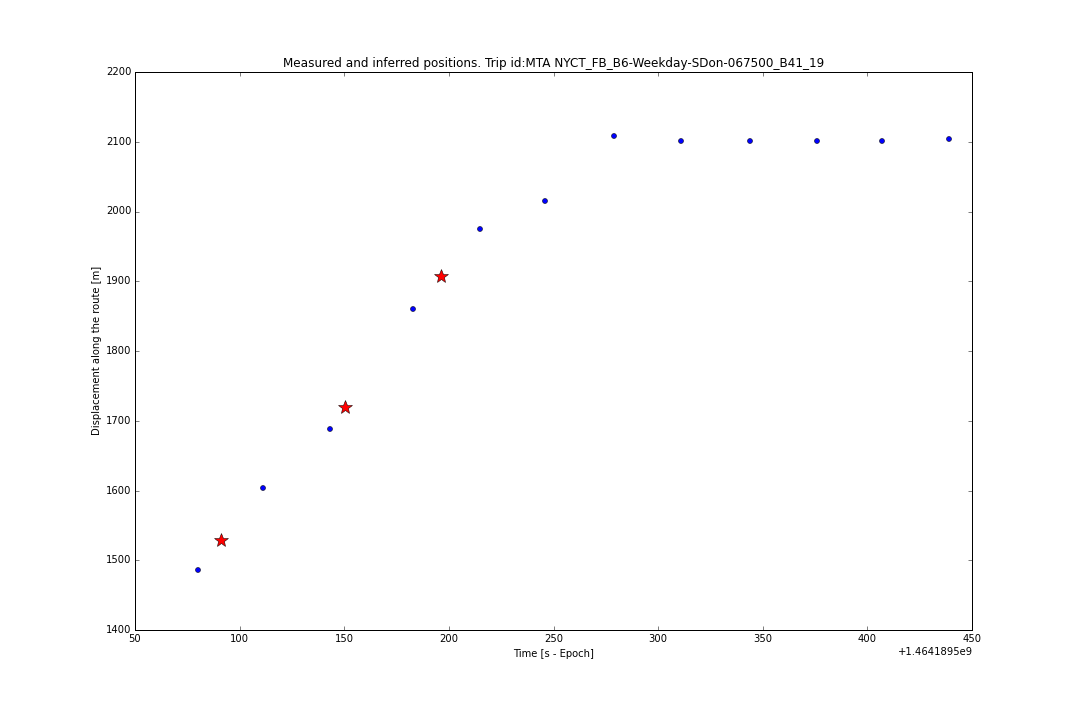
\includegraphics[scale=1.0]{cuteplot.png}






Critical review of reliability metrics



\section{Limitations of the analysis and ways to address these in the future}
Accuracy of the location and time data, when reported, is not in question. However some of the elements are inferred and may cause errors if not handled properly.
Limitations are generally the result of information gaps - specifically when no data is reported where expected.
When no data is reported:
It is unknown if there was actually an operating bus, but a problem arose with hardware or software
If there was a bus (for example, present in earlier and later data), it is possible that the bus did not follow the scheduled route
If there was no bus, the cause is unknown

Trips with data from more than one vehicles - use combination of reported trip\_id and vehicle
Trips with no data - show sensitivity of metrics by assuming trip operated as scheduled
Dwell time
Lacks instantaneous speed information
Schedule metadata
“Disappearing and reappearing bus” 

60-90 second frequency is insufficient for analysis of vehicle behavior on individual street segments and intersections.
30 second frequency is insufficient for measurement of dwell time.
Frequent, long gaps in the data make unbiased performance analysis impossible over full days or date ranges.  Because the gaps tend to arise at the same times each day, any statistical measurement involve time-of-day as an input variable will be biased.  Some analysis may leave time-of-day as an unobserved component of the error term and still show significance in other variables, such as distance-along-trip or street features.
Incomplete reporting of trips may cause bias in calculation of trip-based measurements, such as running time and On Time Performance, if not normalized.
Inferences of points beyond the range of data need to be need to be flagged specially given the possibility that the vehicle did not operate the trip as planned.
If better density is useful, DOT should request the additional elements in the static files provided by MTA


\section{Conclusions and future research}

7.1 Conclusions

7.1.1 Conclusion for the model this project used. (Introduction, Pros and Cons, Bias)
Model for time estimation
Bus time data which is collected by GPS was offered by MTA. The MTA bus GPS database collects the location of each bus every 30 seconds. This project used these data to estimating the departure and arrival time for each stop.
Taking one-year data as this project’s object of study, the data is extremely huge so that big data technology like Spark is widely used in time estimation.
After using spark to deal with the bus time data, this project got a new dataset contained all the information such as the coordinates and timestamp which is more clear and easy for future analyzing.
Measurement for bus performance
After estimating the departure and arrival time for each stop, this project used headways and wait assessment as the measurement to figure out the bus performance and reliability. This will help DOT in future improvement in bus performance and traffic planning.
 In order to make the work easy to share and reproduce, this project choose to use SQL API to manipulate the data, which enable DOT to easily make change by editing the SQL script. 
Method for feature selection

7.1.2 Conclusion for the results this project got. (How the result influence the future operation)
7.1.3 Conclusion for the whole analysis process. (Pros and Cons, Bias, Influence)
Pro:
1. Focus on the viewpoint of DOT, the correlation elements this project chose not only focus on the bus operation, but also other traffic elements.
2. With such large dataset and big data technique, the result of this project’s analysis is more persuasive compared to traditional sample study.
3. Comparison among models(different models to estimate time as well as to measure performance)
Cons:
1. The choice of elements based on formal studies, the objective of which are not all NYC.
2. Too much assumptions.
3. The departure and arrival time for each bus at each stop comes from indirect approximate methods, it is better for MTA to collect the accurate data to help the model works better.
Influence:
The main goal for this project is to figure out the other potential influence factor besides operation to help DOT control and improve bus performance on planning level. Similar methodology and concept could be used in other cities and traffic mode. The big data technology applied in not only traffic analysis but also city wide urban issue offers more reliable result compared with traditional sample studies. 
7.2 Future work
Feature Selection optimization: Pre study and investigation for NYC
Visualization: Use Javascript to create interactive heat map that predicts the chance of delay of specific bus line or stops
Algorithm optimization: Many analyses right now are not computed using big data technique, which means those analyses are hard to applied in large scale such as one year data. In order to analyse quickly in large scale, we must optimize our algorithms to ensure compatibility with big data techniques such as Spark.
Interpolation:
1. Extend sample analysis to all the trips for all the routes in one day.
2. Include the waiting time at stops. Explore previous MTA analysis on Bus Time data to see if   they can provide with a reasonable guess for the dwell time.
3. Compare with the GTFS schedule data to actually implement one of the reliability metrics. It is still unclear if the distance along the route feature is equivalent among both Bus Time and GTF representations.
4. Manage exceptions where there was missing or defectuous data.
5. Apply this analysis for the entire year of Bus Time feed (2015).
6. Consider alternatives for treating deceiving data points at the beginning and end of each trip (“tail” and “head”).
7.3 Further Application
Other cities (need to pay attention to data structure, bus GPS data in some cities collect departure and arrival time instead of location)
Other traffic mode (eg. Subway, city bike. Need to pay attention to the different features of each kinds of traffic mode)





% if have a single appendix:
%\appendix[Proof of the Zonklar Equations]
% or
%\appendix  % for no appendix heading
% do not use \section anymore after \appendix, only \section*
% is possibly needed

% use appendices with more than one appendix
% then use \section to start each appendix
% you must declare a \section before using any
% \subsection or using \label (\appendices by itself
% starts a section numbered zero.)
%


\appendices
\section{Proof of the First Zonklar Equation}
Appendix one text goes here.

% you can choose not to have a title for an appendix
% if you want by leaving the argument blank
\section{}
Appendix two text goes here.


% use section* for acknowledgement
\ifCLASSOPTIONcompsoc
  % The Computer Society usually uses the plural form
  \section*{Acknowledgments}
\else
  % regular IEEE prefers the singular form
  \section*{Acknowledgment}
\fi


The authors would like to thank...


% Can use something like this to put references on a page
% by themselves when using endfloat and the captionsoff option.
\ifCLASSOPTIONcaptionsoff
  \newpage
\fi



% trigger a \newpage just before the given reference
% number - used to balance the columns on the last page
% adjust value as needed - may need to be readjusted if
% the document is modified later
%\IEEEtriggeratref{8}
% The "triggered" command can be changed if desired:
%\IEEEtriggercmd{\enlargethispage{-5in}}

% references section

% can use a bibliography generated by BibTeX as a .bbl file
% BibTeX documentation can be easily obtained at:
% http://www.ctan.org/tex-archive/biblio/bibtex/contrib/doc/
% The IEEEtran BibTeX style support page is at:
% http://www.michaelshell.org/tex/ieeetran/bibtex/
%\bibliographystyle{IEEEtran}
% argument is your BibTeX string definitions and bibliography database(s)
%\bibliography{IEEEabrv,../bib/paper}
%
% <OR> manually copy in the resultant .bbl file
% set second argument of \begin to the number of references
% (used to reserve space for the reference number labels box)
\begin{thebibliography}{1}

\bibitem{IEEEhowto:kopka}
H.~Kopka and P.~W. Daly, \emph{A Guide to {\LaTeX}}, 3rd~ed.\hskip 1em plus
  0.5em minus 0.4em\relax Harlow, England: Addison-Wesley, 1999.

\end{thebibliography}

% biography section
% 
% If you have an EPS/PDF photo (graphicx package needed) extra braces are
% needed around the contents of the optional argument to biography to prevent
% the LaTeX parser from getting confused when it sees the complicated
% \includegraphics command within an optional argument. (You could create
% your own custom macro containing the \includegraphics command to make things
% simpler here.)
%\begin{IEEEbiography}[{\includegraphics[width=1in,height=1.25in,clip,keepaspectratio]{mshell}}]{Michael Shell}
% or if you just want to reserve a space for a photo:

\begin{IEEEbiography}{Michael Shell}
Biography text here.
\end{IEEEbiography}

% if you will not have a photo at all:
\begin{IEEEbiographynophoto}{John Doe}
Biography text here.
\end{IEEEbiographynophoto}

% insert where needed to balance the two columns on the last page with
% biographies
%\newpage

\begin{IEEEbiographynophoto}{Jane Doe}
Biography text here.
\end{IEEEbiographynophoto}

% You can push biographies down or up by placing
% a \vfill before or after them. The appropriate
% use of \vfill depends on what kind of text is
% on the last page and whether or not the columns
% are being equalized.

%\vfill

% Can be used to pull up biographies so that the bottom of the last one
% is flush with the other column.
%\enlargethispage{-5in}



% that's all folks
\end{document}

